\section{Modelado predictivo}

En esta sección, se presenta el modelado predictivo realizado para clasificar los datos según el nivel de contaminación. Para ello, se empleó la librería de Python LazyPredict\cite{LazyPredict}, la cual nos permitió identificar qué modelo presenta la mejor exactitud sobre un conjunto de datos de muestra.

\begin{figure}[htb] 
    \begin{center} 
        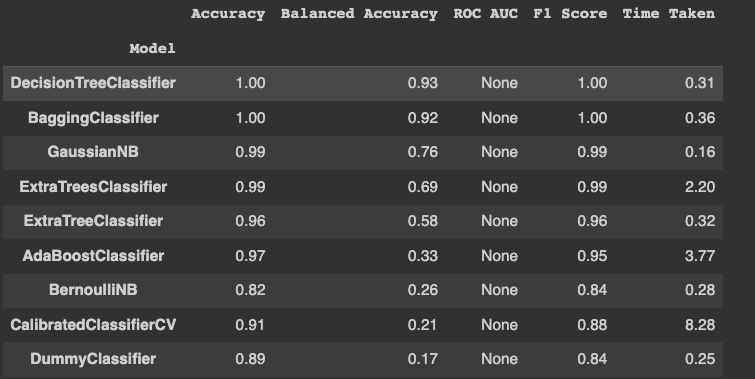
\includegraphics[width=8cm]{Papper IB/Images/model_1.png}
    \end{center} 
    \caption{Salida de LazyPredictor} 
    \label{fig:fig4} 
\end{figure} 

El análisis de LazyPredictor nos indica que se recomienda utilizar un modelo basado en Árbol de decisión (DecisionTreeClassifier). A continuación, se procedió a entrenar el modelo utilizando este algoritmo y posteriormente se analizaron las métricas obtenidas.

El modelo fue entrenado inicialmente sin especificar los hiperparámetros del Árbol de decisión, tales como max\_depth, min\_samples\_leaf y min\_samples\_split. Los resultados obtenidos se muestran en la siguiente figura:

\begin{figure}[htb] 
    \begin{center} 
        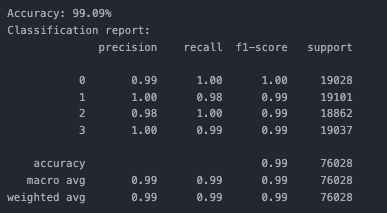
\includegraphics[width=8cm]{Papper IB/Images/model_2.png}
    \end{center} 
    \caption{Reporte de clasificación} 
    \label{fig:fig2} 
\end{figure} 

A partir de los resultados presentados en el reporte, se pueden extraer diversas conclusiones relevantes.

En primer lugar, el modelo obtuvo una precisión del 99.09\%, lo cual indica que fue capaz de clasificar correctamente el 99.09\% de las instancias en el conjunto de datos. Esta alta precisión evidencia la capacidad del modelo para realizar una clasificación confiable del nivel de contaminación.\cite{xu2017long}

El reporte de clasificación también incluye métricas como recall y F1-Score para cada clase. Estas métricas proporcionan información adicional sobre la capacidad del modelo para identificar correctamente las instancias positivas y negativas. En general, se observa que el modelo obtuvo valores elevados de recall y F1-Score para todas las clases. Esto indica que el modelo logró identificar la mayoría de las instancias reales de cada clase y alcanzó un equilibrio entre precisión y recall.\cite{liang2018analysis}

Además, es relevante destacar que el modelo fue evaluado en un conjunto de datos de considerable tamaño, con un total de 76,028 instancias. Esta cantidad de datos aumenta la confianza en los resultados y sugiere que el modelo ha sido probado en un escenario realista.

\subsection{Validación cruzada}

La validación cruzada es una técnica esencial para evaluar el rendimiento del modelo de manera robusta. En este caso, se realizó una validación cruzada y se obtuvieron los siguientes datos:

\textbf{Mejores parámetros:}
\begin{itemize}
    \item max\_depth: None
    \item min\_samples\_leaf: 1
    \item min\_samples\_split: 2
\end{itemize}

\textbf{Puntuaciones de validación cruzada:}
\begin{itemize}
    \item [0.99019166, 0.98928974, 0.99036077, 0.99007892, 0.99024803, 0.99126268, 0.99013473, 0.99086758, 0.98945826, 0.98844354]
\end{itemize}

\textbf{Puntuación promedio de validación cruzada:} 0.990033590214823

\textbf{Exactitud:} 99.10\%

Estos resultados confirman y respaldan el desempeño del modelo de Árbol de decisión en la clasificación del nivel de contaminación. La obtención de una puntuación promedio de validación cruzada alta indica que el modelo es consistente y generaliza bien en diferentes subconjuntos de datos, esto también se puede evidenciar en la matriz de confusión\\ 
\begin{figure}[htb] 
    \begin{center} 
        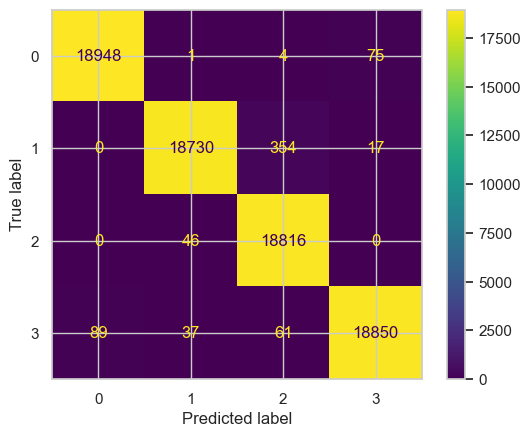
\includegraphics[width=8cm]{Papper IB/Images/model_3.png}
    \end{center} 
    \caption{Matriz de confusión} 
    \label{fig:fig2} 
\end{figure} 


En conclusión, el modelo de Árbol de decisión ha demostrado ser altamente efectivo en la clasificación del nivel de contaminación. Los resultados obtenidos, respaldados por las métricas de evaluación y la validación cruzada, indican que el modelo es confiable y preciso en su capacidad para clasificar correctamente el nivel de contaminación en función de los datos proporcionados. Estos resultados son alentadores y sugieren la aplicabilidad del modelo en situaciones reales relacionadas con la clasificación de la contaminación.\cite{li2017study}

Finalmente una metrica muy importante es comprender si el modelo tiene overfitting o underfitting, eso se puede visualizar en la siguiente grafica: 
\begin{figure}[htb] 
    \begin{center} 
        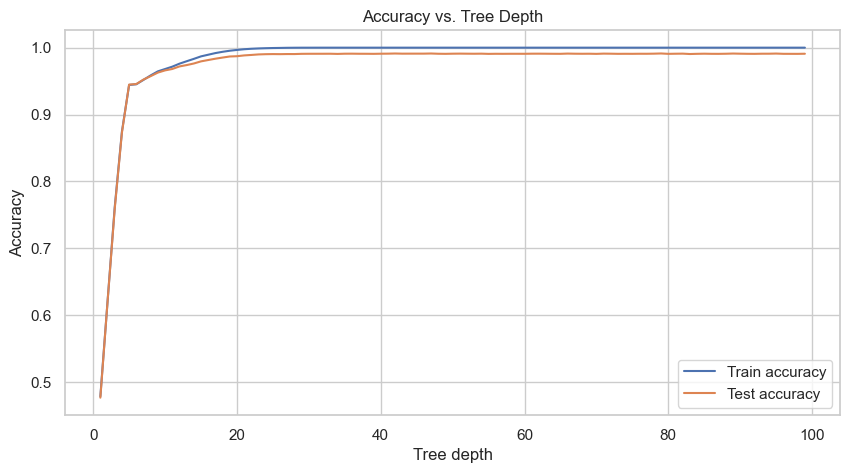
\includegraphics[width=8cm]{Papper IB/Images/model_4.png}
    \end{center} 
    \caption{Matriz de confusión} 
    \label{fig:fig1} 
\end{figure} 
